\documentclass[a4paper,12pt]{article}

% Package for better font and formatting options
\usepackage{lipsum}
\usepackage[colorlinks=true, linkcolor=blue, urlcolor=blue]{hyperref}
\usepackage{graphicx}


% Title and author information
\title{Axis Dome Camera - Video Authentication}
\author{Mohammed Rahman}
\date{\today}

\begin{document}
% Creates title section
\maketitle

\tableofcontents

\newpage
% Introduction section
\section{Setup}
The setup documented follows the steps listed on the \href{https://help.axis.com/en-us/axis-p3265-lve}{datasheet}. A Windows-based system was used to locate the IP address of the Axis Dome camera and setup shared storage, while a Linux-based system was used for the rest of the project.\\ \\The camera is currently configured with factory settings, including the default IP address. To locate the IP address, use either AXIS Utility or the Axis Device Manager. In this demonstration, AXIS Utility was used. When AXIS IP Utility is opened and the camera is connected, it should automatically detect the camera. The camera's IP address will be displayed on the left-hand side. Copy this address into a browser to access the camera software. \\

\noindent The details for the account are:\\[1em]
\textbf{User:} \texttt{root}\\
\textbf{Password:} \texttt{Electronic1} \\ 

\noindent To turn on video signing from this window, navigate to \texttt{Video} \(\to\) \texttt{Stream} \(\to\) \texttt{General}.

\section{Network Storage}

There are two types of storage available: network storage and SD cards. The former was chosen. \\

First, a shared folder will need to be created on the Windows machine (this can be done on Linux too), which can be done by following this \href{https://bdsdoc.com/kb-articles/how-to-create-a-network-shared-folder/}{guide}. Then, obtain the IP address of the machine hosting the shared folder. This can be done with: \\

\noindent \textbf{Windows:} \texttt{ipconfig}\\
\textbf{Linux:}  \texttt{ip a} \\

Navigate to \texttt{System} \(\to\) \texttt{Storage} \(\to\) \texttt{Add Network Storage}. Enter the IP address of the host machine, along with the host's username, password, and the path to the shared folder. Leave all other settings at their default values.

\section{Video Signing}

AXIS cameras can utilise \href{https://www.axis.com/dam/public/0e/54/e6/axis-edge-vault-en-US-419338.pdf}{AXIS Edge Vault} to sign videos. Ensure that the cameras in use have up-to-date firmware to enable video signing, as cameras straight from the box may not support this functionality. The process of video signing is outlined on pages 13 to 16 of the \href{https://help.axis.com/en-us/axis-p3265-lve}{datasheet}.

\section{Framework Dependencies}

The signed-video-framework requires several dependencies, which are listed below and can be found on their \href{https://github.com/AxisCommunications/signed-video-framework}{GitHub}:

\begin{itemize}
    \item \texttt{meson}
    \item \texttt{ninja}
    \item \texttt{OpenSSL}
    \item \texttt{libcheck}
\end{itemize}

To run the two applications, \texttt{signer} and \texttt{validator}, \texttt{GStreamer} will also be needed.

\subsection{Meson and ninja}

To install both \texttt{meson} and \texttt{ninja}, use the following commands:

\begin{verbatim}
    $ pip install meson
    $ pip install ninja
\end{verbatim}

\subsection{OpenSSL}

To install \texttt{OpenSSL}, use the following commands:

\begin{verbatim}
    $ git clone https://github.com/openssl/openssl
    $ cd path/to/cloned/repo
    $ ./Configure 
    $ make 
    $ make test
\end{verbatim}

If the tests do not pass, you may need to run the commands by prepending \texttt{sudo}.

\subsection{libcheck}

To install \texttt{libcheck}, run the following command:

\begin{verbatim}
    $ sudo apt-get install check
\end{verbatim}

\subsection{GStreamer}

To install \texttt{GStreamer}, run the following command: \\

\noindent
\texttt{\$ apt-get install libgstreamer1.0-dev} \\
\texttt{libgstreamer-plugins-base1.0-dev} \\
\texttt{libgstreamer-plugins-bad1.0-dev} \\
\texttt{gstreamer1.0-plugins-base} \\
\texttt{gstreamer1.0-plugins-good} \\
\texttt{gstreamer1.0-plugins-bad} \\
\texttt{gstreamer1.0-plugins-ugly} \\
\texttt{gstreamer1.0-libav} \\
\texttt{gstreamer1.0-tools} \\
\texttt{gstreamer1.0-x} \\
\texttt{gstreamer1.0-alsa} \\
\texttt{gstreamer1.0-gl} \\
\texttt{gstreamer1.0-gtk3} \\
\texttt{gstreamer1.0-qt5} \\
\texttt{gstreamer1.0-pulseaudio}

\section{Framework}
Both the \href{https://github.com/AxisCommunications/signed-video-framework}{signed-video-framework} and \href{https://github.com/AxisCommunications/signed-video-framework-examples}{signed-video-framework-examples} repositories were cloned under the same parent directory. All subsequent commands in the framework, as well as those for the \texttt{validator} and \texttt{signer} sections, were run in the parent directory. \\

The framework supports both H.264 and H.265 encoding. Depending on the encoding type, the appropriate format should be used in the signer and validator commands. \\

To compile the framework to the run the two apps, use the following commands:

\begin{verbatim}
    $ meson --prefix $PWD/local_install signed-video-framework 
      build
    $ ninja -C build
    $ meson install -C build 
    $ ninja -C build test 
\end{verbatim}

The unit tests should all pass if done correctly.

\section{Signer}
The commands listed below used to compile the validator can also be found on the \href{https://github.com/AxisCommunications/signed-video-framework-examples/tree/master/apps/signer}{AXIS Signer GitHub}. \\

If the camera does not automatically perform the signing, the signer step can be done manually. To do this, you must first compile the signer by following the commands provided below:

\begin{verbatim}
    $ export GST_PLUGIN_PATH=$PWD/my_installs
    $ meson --prefix $PWD/my_installs -Dsigner=true signed-
      video-framework-examples build_signer 
    $ meson install -C build_signer
\end{verbatim}

The \texttt{GST\_PLUGIN\_PATH} environment variable must be set to the local installation directory, as the signer application is implemented as a GStreamer element. \\

If the signer application is compiled successfully, it will be located in \texttt{local\_install/bin/signer}. \\

To run the signer on a test file, first copy the test file into the same directory where the command is executed. In this case, the file should be placed in the parent directory:

\begin{verbatim}
    $ ./local_install/bin/signer -c h264 test_h264.mp4 
\end{verbatim}

If the signer is successful, a new file with the prefix \texttt{signed\_} should be generated.

\section{Validator}

The commands listed below used to compile the validator can also be found on the \href{https://github.com/AxisCommunications/signed-video-framework-examples/tree/master/apps/validator}{AXIS Validator GitHub}. 

\begin{verbatim}
    $ meson --prefix $PWD/local_install -Dvalidator=true signed-
      video-framework-examples build_validator
    $ meson install -C build_validator
\end{verbatim}

If the validator application is compiled successfully, it will be located in \texttt{local\_install/bin/validator}. \\

To run the validator on a test file, first copy the test file into the same directory where the command is executed. In this case, the file should be placed in the parent directory:

\begin{verbatim}
    $ ./local_install/bin/validator -c h264 test_h264.mp4 
\end{verbatim}

The results can be viewed in the \texttt{validation\_results} text file produced.

\section{Product Information}

Figure 1 below illustrates the product information as displayed by the validator.

\begin{figure}[h!]
    \centering
    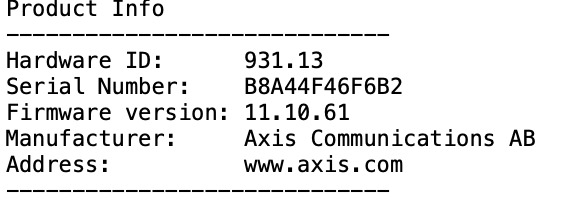
\includegraphics[width=0.8\textwidth]{IN.jpeg}
    \caption{Product information displayed by the validator.}
    \label{fig:axis-dome-example}
\end{figure}

The validator retrieves this information from the metadata, which is stored within the MKV file, as demonstrated in Figure 2. 

\begin{figure}[h!]
    \centering
    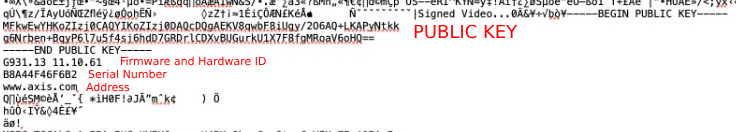
\includegraphics[width=1\textwidth]{FIEL.png}
    \caption{Metadata stored within the MKV file.}
    \label{fig:axis-dome-example}
\end{figure}

However, the "manufacturer" field could not be located in the MKV file when opened as a text file. To find the manufacturer, Hex Fiend was used to decode sections of the video stream as shown below.

\begin{figure}[h!]
    \centering
    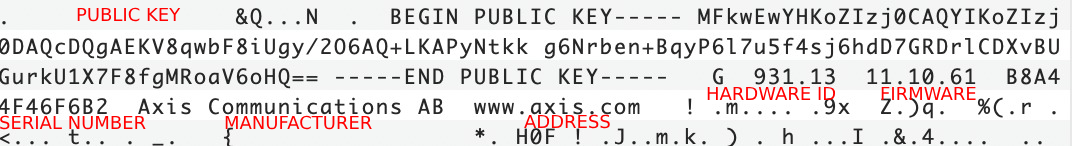
\includegraphics[width=1\textwidth]{K.png}
    \caption{MKV file decoded using Hex Fiend.}
    \label{fig:axis-dome-example}
\end{figure}

This indicates the "manufacturer" field is embedded within the video stream.

\newpage

\section{Findings}

\subsection{Validating Non-Tampered Camera Footage}
Figure 4 below demonstrates running the validator on a signed video captured by the AXIS Dome camera.

\begin{figure}[h!]
    \centering
    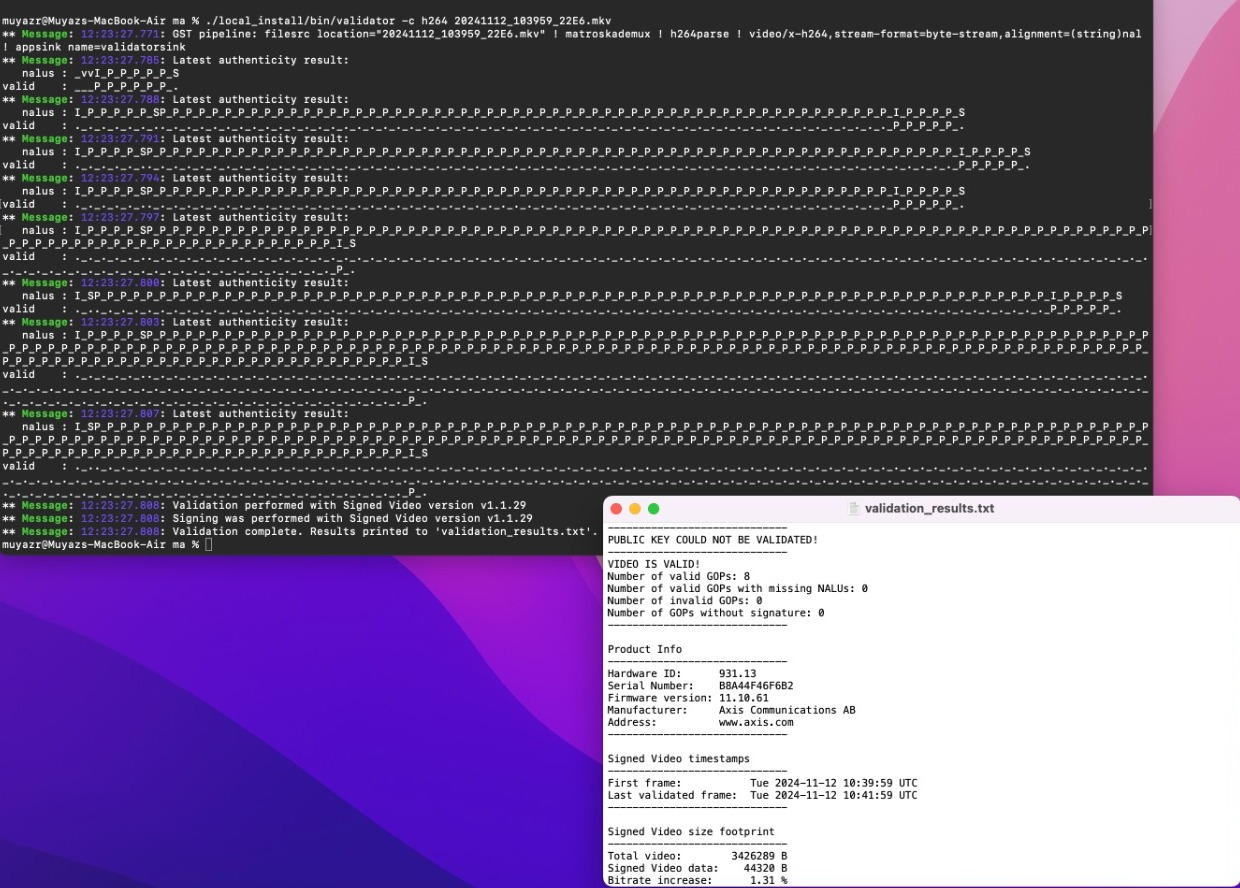
\includegraphics[width=1\textwidth]{pic.jpeg}
    \caption{Running the validator on a signed video from the AXIS Dome camera.}
    \label{fig:axis-dome-example}
\end{figure}

As shown in Figure 4, the video is validated, indicating that both the public key is valid and the video has not been tampered with. This aligns with our expectations. However, it also shown that the public key cannot be validated. This means the validator is unable to confirm the authenticity of the public key itself. As stated by the developers on GitHub, this is outside the scope of the framework's purpose: \\

\begin{quote}
    "The framework signals the video as authentic, assuming the public key can be trusted. Validating the public key is out of scope."
\end{quote}

Possible solutions to address this issue include validating the public key through a Certificate Authority or implementing a lookup system to verify whether the public key in question is included in a trusted collection of public keys.

\subsection{Validating Tampered Camera Footage}

A PNG image was inserted into the signed video from the above section. This was accomplished using \texttt{ffmpeg} with the following command:

\begin{verbatim}
    $ ffmpeg -i input_video.mkv -i image.png -filter_complex 
      "overlay=x=10:y=10" -c:a copy output_video.mkv
\end{verbatim}

Figure 5 below shows the result of running the validator on this altered signed video captured by the AXIS Dome camera.

\begin{figure}[h!]
    \centering
    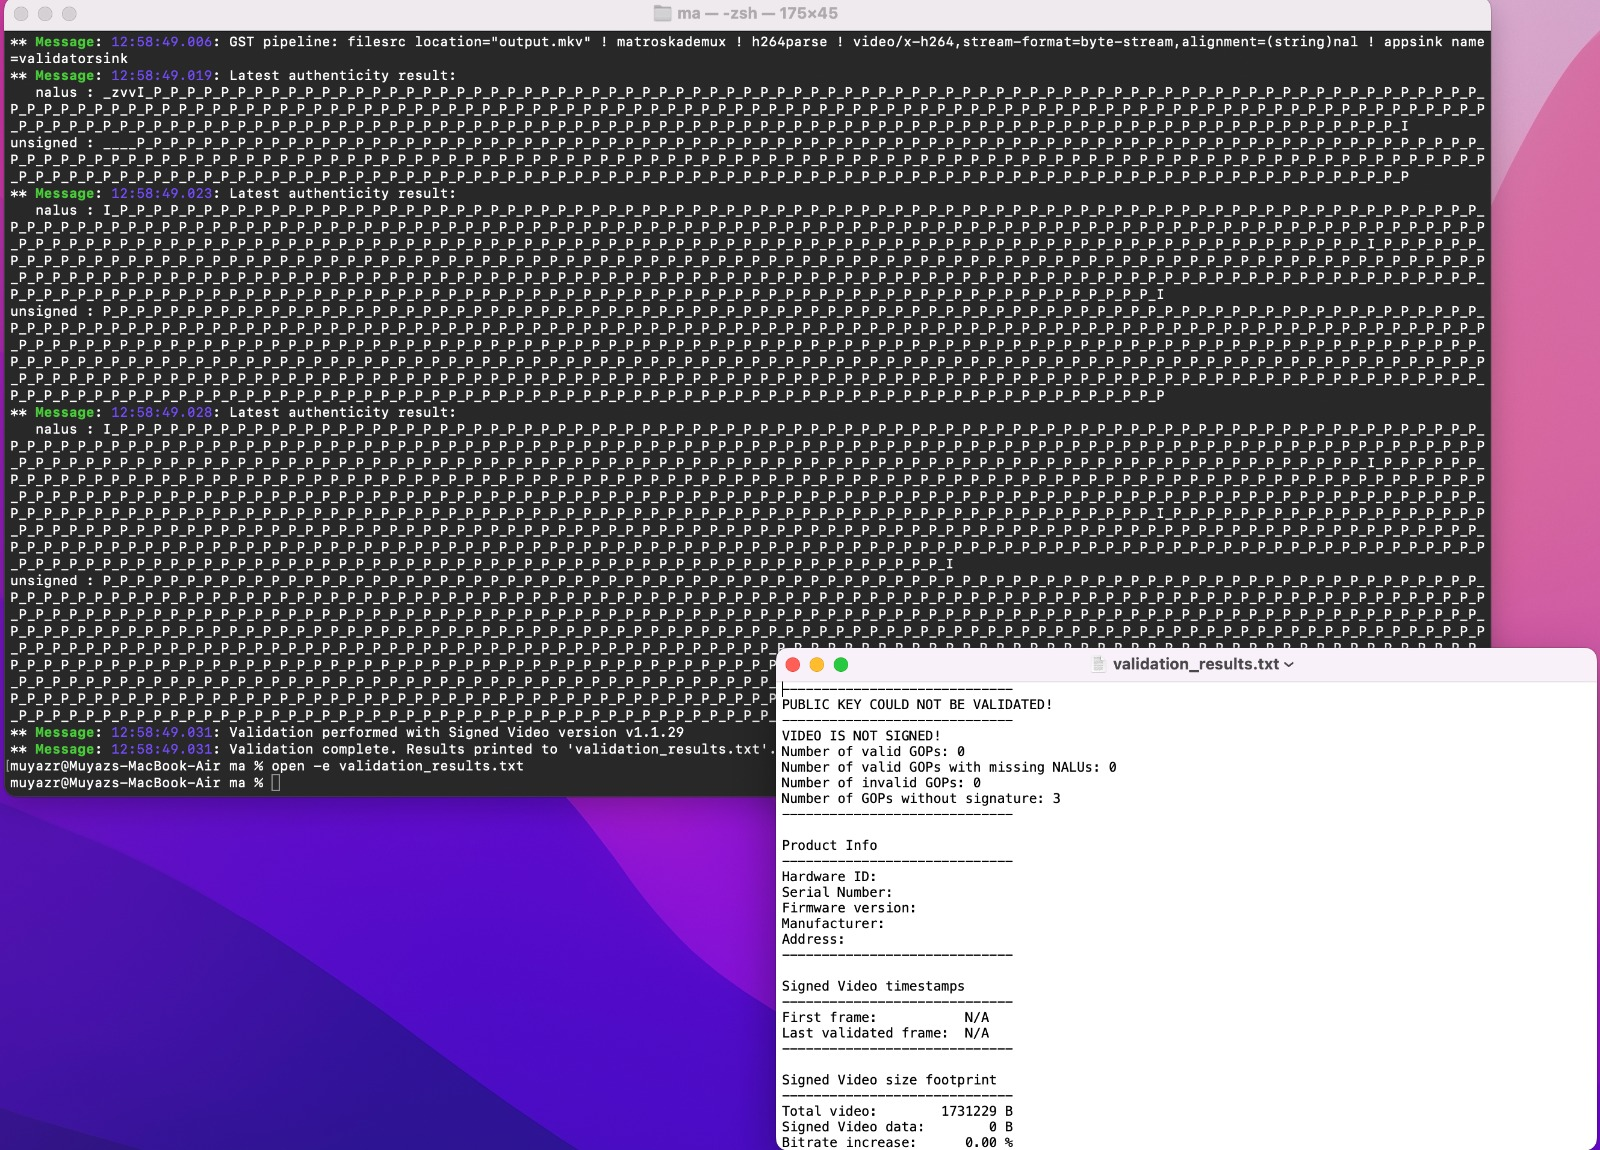
\includegraphics[width=1\textwidth]{pic1.jpg}
    \caption{Running the validator on a tampered signed video from the AXIS Dome camera.}
    \label{fig:axis-dome-example}
\end{figure}

Once again, the public key could not be validated. The validator correctly rejected the video, but it was not marked as invalid. Instead, the video was labeled as "not signed" rather than "invalid". \\ 

I believe this issue arises from the video being altered. In the original signed video, there were 8 signed GOPs (Group of Pictures), whereas the altered video shows only 3 unsigned GOPs. However, I don't see this as a problem because all the videos produced by the AXIS Dome camera are expected to be signed. If the validator returns "unsigned," it clearly indicates that the video has been tampered with.

\end{document}

